\documentclass{exam}
%\documentclass[answers]{exam}
\hbadness=99999
\usepackage[total={6.5in,9in}]{geometry}

\usepackage{enumerate}
\usepackage{amsmath}
\usepackage[table]{xcolor}
\usepackage{graphicx}
\usepackage{tikz}
%\usepackage{pgfplots}
\usepackage{multicol}

% for syntax highlighting
\usepackage{minted}
\usemintedstyle[cpp]{xcode}

% for overlay of output
\usepackage[overlay,showboxes]{textpos}

\pagestyle{plain}

\setlength\columnsep{50pt}
\newcommand{\key}{\hfill
      \raisebox{-.3\height}{\includegraphics[width=0.6in]{figures/key.png}}}

\begin{document}
  \thispagestyle{empty}
  \setlength{\parindent}{0pt}

  \begin{center}
    \Large Activity \#6: Version Control \\[5pt]
    \large Recorder's Report\\[20pt]
    \normalsize
    \begin{tabular}{lrp{0.1in}lr}
      Manager:  & \fillin[][2.0in] & & Presenter: & \fillin[][2.0in]\\[15pt]
      Recorder: & \fillin[][2.0in] & & Driver:    & \fillin[][2.0in]\\[15pt]
      Date:     & \fillin[][2.0in] & & Score:     & Satisfactory \hspace{10pt} /
      \hspace{10pt} Not Satisfactory
    \end{tabular}
  \end{center}
  \par\vskip 15pt
  
  Record your group's answers to the key questions (marked with
  \raisebox{-.3\height}{\includegraphics[width=0.5in]{figures/key.png}})
  below.
  \begin{enumerate}[(a)]
    \itemsep 2.5in
    \item Model 1, Question \#4
    \item Model 2, Question \#8
  \end{enumerate}

  \clearpage\pagenumbering{arabic} 
  
  \begin{center}
    \Large Activity \#6: Version Control \\[5pt]
    \large Activity Guide\\[20pt]
  \end{center}

  \begin{center}
    \fbox{
      \begin{minipage}{5.5in}
        {\bf Learning Objectives:} Students will be able to:
        \begin{itemize}
          \item Content:\\[-20pt]
            \begin{itemize}
              \itemsep 0pt
              \item Explain the core VCS concepts of {\it checking
                out}, {\it updating}, {\it branching}, and {\it merging}
              \item Describe an effective workflow for a VCS
            \end{itemize}
          \item Process\\[-20pt]
            \begin{itemize}
              \itemsep 0pt
              \item Construct timeline diagrams depicting various
                interactions with a VCS\\[-5pt]
            \end{itemize}
        \end{itemize}
      \end{minipage}
      }
  \end{center}
  \par\vskip 10pt
  
  
  {\bf\large Model 1: Version Control Scenarios}\\[-5pt]
  \begin{center}
    \small
    \begin{tabular}{p{1.25in}p{1.75in}p{2.25in}}
      \begin{minipage}{1.25in}
        \centering
        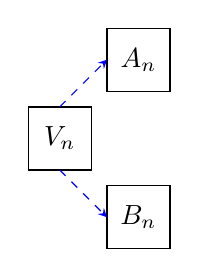
\begin{tikzpicture}[scale=0.8]
          \draw (0,0) rectangle (1,1);
          \node at (0.5,0.5) {$V_n$};
          \draw (1.25,1.25) rectangle (2.25,2.25);
          \node at (1.75,1.75) {$A_n$};
          \draw (1.25,-0.25) rectangle (2.25,-1.25);
          \node at (1.75,-0.75) {$B_n$};
          \draw[blue,dashed,-stealth] (0.5,1) -- (1.25,1.75);
          \draw[blue,dashed,-stealth] (0.5,0) -- (1.25,-0.75);
        \end{tikzpicture}\par
        Scenario \#1
      \end{minipage}
      &
      \begin{minipage}{1.75in}
        \centering
        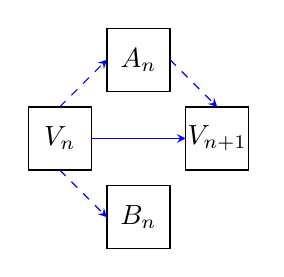
\begin{tikzpicture}[scale=0.8]
          \draw (0,0) rectangle (1,1);
          \node at (0.5,0.5) {$V_n$};
          \draw (1.25,1.25) rectangle (2.25,2.25);
          \node at (1.75,1.75) {$A_n$};
          \draw (1.25,-0.25) rectangle (2.25,-1.25);
          \node at (1.75,-0.75) {$B_n$};
          \draw (2.5,0) rectangle (3.5,1);
          \node at (3,0.5) {$V_{n+1}$};
          \draw[blue,dashed,-stealth] (0.5,1) -- (1.25,1.75);
          \draw[blue,dashed,-stealth] (0.5,0) -- (1.25,-0.75);
          \draw[blue,dashed,-stealth] (2.25,1.75) -- (3,1);
          \draw[blue,-stealth] (1,0.5) -- (2.5,0.5);
        \end{tikzpicture}\par
        Scenario \#2
      \end{minipage}
      &
      \begin{minipage}{2.25in}
        \centering
        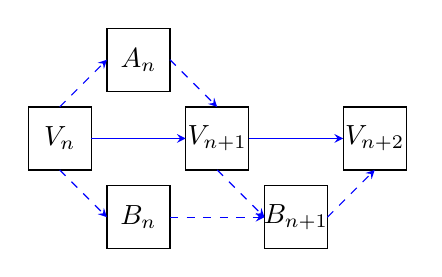
\begin{tikzpicture}[scale=0.8]
          \draw (0,0) rectangle (1,1);
          \node at (0.5,0.5) {$V_n$};
          \draw (1.25,1.25) rectangle (2.25,2.25);
          \node at (1.75,1.75) {$A_n$};
          \draw (1.25,-0.25) rectangle (2.25,-1.25);
          \node at (1.75,-0.75) {$B_n$};
          \draw (2.5,0) rectangle (3.5,1);
          \node at (3,0.5) {$V_{n+1}$};
          \draw (3.75,-0.25) rectangle (4.75,-1.25);
          \node at (4.25,-0.75) {$B_{n+1}$};
          \draw (5,0) rectangle (6,1);
          \node at (5.5,0.5) {$V_{n+2}$};
          \draw[blue,dashed,-stealth] (0.5,1) -- (1.25,1.75);
          \draw[blue,dashed,-stealth] (0.5,0) -- (1.25,-0.75);
          \draw[blue,dashed,-stealth] (2.25,1.75) -- (3,1);
          \draw[blue,-stealth] (1,0.5) -- (2.5,0.5);
          \draw[blue,dashed,-stealth] (2.25,-0.75) -- (3.75,-0.75);
          \draw[blue,dashed,-stealth] (3,0) -- (3.75,-0.75);
          \draw[blue,dashed,-stealth] (4.75,-0.75) -- (5.5,0);
          \draw[blue,-stealth] (3.5,0.5) -- (5,0.5);
        \end{tikzpicture}\par
        Scenario \#3
      \end{minipage}
    \end{tabular}
  \end{center}
  \par\vskip 5pt
  
  {\it\large Refer to Model 1 above as your group develops consensus answers
    to the questions below.}
    \par\vskip 10pt
    
  \begin{enumerate}
    \itemsep 20pt
    
    \item A {\it version control system} (VCS) helps to manage
      multiple versions of files, such as program source code.  Such a
      collection of files is called a {\it repository}.  In the
      model above, $V_n$ represents the current version of the
      repository. If Amy and Bob are two developers working on the code
      stored in $V_n$, they will first {\it check out} their own local copies,
      $A_n$ and $B_n$, of the repository to edit. The first scenario of
      the model depicts this situation.
      \par\vskip 10pt
      \begin{enumerate}
        \item What do the dashed arrows represent?
          \begin{solution}[0.75in]
            The dashed lines represent a checkout or copy of the repository
            to edit in a local environment.
          \end{solution}
        \item Why is it better for Amy and Bob to edit their own copies
          of the repository rather than files in $V_n$ directly?
          \begin{solution}[1in]
            As developers make changes the code will likely be broken, so 
            it is better for changes not to be visible to others till the
            development and testing process is done.
          \end{solution}
        \item What problems might result from Amy and Bob editing
          their own copies of the repository?
          \begin{solution}[0.75in]
            They will not get changes (fixes and features) added by others, 
            so the changes they make will not be compatible with the current
            version in the repository.
          \end{solution}
      \end{enumerate}
      
    \item After editing, Amy adds her changes to the main repository
      to create a new version, $V_{n+1}$.  We say that Amy
      {\it commits} changes to the repository.  This is shown in
      the second scenario.
      \par\vskip 10pt
      \begin{enumerate}
        \item How is Amy's commit shown in the diagram for scenario \#2?
          \begin{solution}[0.75in]
            There are dashed lines from Amy's copy to the new version and
            a solid line from the previous version to the new version.
          \end{solution}
        \item Before Amy commits her code, can Bob view Amy's changes?
          Explain.
          \begin{solution}[0.75in]
            Amy's edits are in Amy's environment, not in the shared 
            repository. So, no, Bob cannot view Amy's changes (unless he 
            has access to Amy's environment through other means).
          \end{solution}
        \item Why is it important that Amy test her code before she
          commits it?
          \begin{solution}[0.75in]
            Once Amy commits her code to the shared repository, then other 
            developers will start using it. If it is broken then other 
            developers will be impacted.
          \end{solution}
      \end{enumerate}
      
    \item Before Bob can commit his changes, he must get all of Amy's
      changes from $V_{n+1}$.  We say that Bob {\it updates} his local
      copy from the repository.  This is depicted in the third scenario.
      \par\vskip 10pt
      \begin{enumerate}
        \item Why must Bob update his local copy before he can commit
          changes to the repository?
          \begin{solution}[0.75in]
            Bob should make sure that he does not accidentally overwrite
            or replace Amy's changes. He should also make sure that his 
            changes are compatible with Amy's changes. It could be that 
            Amy's changes work in isolation, and Bob's changes work in 
            isolation, but together they do not work. 
          \end{solution}
        \item Why are there two arrows pointing to $B_{n+1}$, Bob's
          updated copy of the repository, instead of one?
          \begin{solution}[0.75in]
            Bob's new copy has changes from both sources.
          \end{solution}
        \item What should Bob do before he commits his updated changes
          back to the main repository?
          \begin{solution}[0.75in]
            Bob should review Amy's changes to see if they conflict with 
            his changes. Bob should also thoroughly test the merged code.
          \end{solution}
      \end{enumerate}
      
    \item Which of the operations discussed in this model ({\it
      checkout}, {\it commit}, and {\it update}) are best\key\\[-2.5mm] described
      by the following?
      \par\vskip 15pt
      \begin{enumerate}
        \itemsep 15pt
        \item Transfers the most amount of data:
          \hfill \fillin[checkout][2.5in]
        \item Transfers the least amount of data:
          \hfill \fillin[commit (an update may have several commits)][2.5in]
        \item Might result in a {\it conflict} between file versions:
          \hfill \fillin[update (or a commit without an update)][2.5in]
      \end{enumerate}
      
    \item We can use {\it timeline diagrams} such as those shown in the
      model to visualize versions ({\it nodes} represented by
      rectangles) and connections ({\it links} represented by arrows). 
      Draw a timeline diagram to show the following sequence of events.
      \begin{center}
        \begin{minipage}{4.5in}
          \begin{enumerate}[i.]
            \itemsep -2pt
            \item We start with version 10 of the project files
            \item Amy checks out her own copy
            \item Amy edits and commits, creating a new version
            \item Bob checks out his own copy            
            \item Amy makes another edit and commits again
            \item Bob updates
            \item Bob edits and commits
          \end{enumerate}
        \end{minipage}
      \end{center}
      \par\vskip 15pt
      \begin{solution}[2in]
      \end{solution}
      

  {\bf\large Model 2: Branching and Merging}\\[-5pt]
  \begin{center}
    \begin{tabular}{p{2.5in}p{2.5in}}
      \begin{minipage}{2.5in}
        \centering
        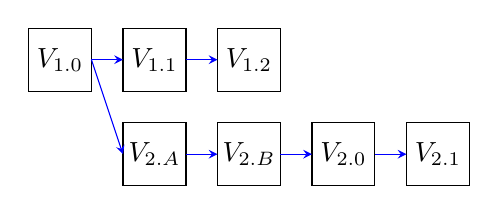
\begin{tikzpicture}[scale=0.8]    
          \draw (0,0) rectangle (1,1);
          \node at (0.5,0.5) {$V_{1.0}$};
          \draw (1.5,0) rectangle (2.5,1);
          \node at (2,0.5) {$V_{1.1}$};
          \draw (3,0) rectangle (4,1);
          \node at (3.5,0.5) {$V_{1.2}$};
          \draw (1.5,-0.5) rectangle (2.5,-1.5);
          \node at (2,-1) {$V_{2.A}$};
          \draw (3,-0.5) rectangle (4,-1.5);
          \node at (3.5,-1) {$V_{2.B}$};
          \draw (4.5,-0.5) rectangle (5.5,-1.5);
          \node at (5,-1) {$V_{2.0}$};
          \draw (6,-0.5) rectangle (7,-1.5);
          \node at (6.5,-1) {$V_{2.1}$};      
          \draw[blue,-stealth] (1,0.5) -- (1.5,0.5);
          \draw[blue,-stealth] (1,0.5) -- (1.5,-1);
          \draw[blue,-stealth] (2.5,0.5) -- (3,0.5);
          \draw[blue,-stealth] (2.5,-1) -- (3,-1);
          \draw[blue,-stealth] (4,-1) -- (4.5,-1);
          \draw[blue,-stealth] (5.5,-1) -- (6,-1);
        \end{tikzpicture}\par
        Scenario \#1
      \end{minipage}
      &
      \begin{minipage}{2.5in}
        \centering
        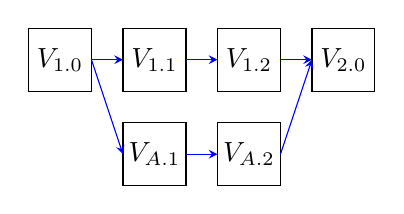
\begin{tikzpicture}[scale=0.8]    
          \draw (0,0) rectangle (1,1);
          \node at (0.5,0.5) {$V_{1.0}$};
          \draw (1.5,0) rectangle (2.5,1);
          \node at (2,0.5) {$V_{1.1}$};
          \draw (3,0) rectangle (4,1);
          \node at (3.5,0.5) {$V_{1.2}$};
          \draw (4.5,0) rectangle (5.5,1);
          \node at (5,0.5) {$V_{2.0}$};
          \draw (1.5,-0.5) rectangle (2.5,-1.5);
          \node at (2,-1) {$V_{A.1}$};
          \draw (3,-0.5) rectangle (4,-1.5);
          \node at (3.5,-1) {$V_{A.2}$};
          \draw[blue,-stealth] (1,0.5) -- (1.5,0.5);
          \draw[blue,-stealth] (2.5,0.5) -- (3,0.5);
          \draw[blue,-stealth] (4,0.5) -- (4.5,0.5);
          \draw[blue,-stealth] (1,0.5) -- (1.5,-1);
          \draw[blue,-stealth] (2.5,-1) -- (3,-1);
          \draw[blue,-stealth] (4,-1) -- (4.5,0.5);
        \end{tikzpicture}\par
        Scenario \#2
      \end{minipage}
    \end{tabular}
  \end{center}
  
  {\it\large Refer to Model 2 above as your group develops consensus answers
    to the questions below.}
    \par\vskip 10pt
    
      \item After an initial version of a program is finished,
        you may wish to start working on new features without breaking
        the existing version. Versions that have not yet been released 
        are sometimes labeled with the names alpha and beta. 
        You may then continue to make small bug fixes
        to the existing version in parallel with the major changes
        being made to the new version.  These parallel versions of the
        software are called {\it branches} and creating a new parallel
        version is called {\it branching}.
        \par\vskip 10pt
        \begin{enumerate}
          \item Identify the initial version of the repository
            shown in scenario \#1 of the model along with the versions
            that are bug fixes of that initial version.
            \begin{solution}[0.75in]
              {$V_{1.0}$}, {$V_{1.1}$}, and {$V_{1.2}$}
            \end{solution}
          \item How are versions {$V_{1.0}$} and {$V_{2.A}$} of this first scenario related?
            \begin{solution}[0.5in]
              They are essentially the same; {$V_{2.A}$} is a copy of {$V_{1.0}$} 
              to which no changes have yet been applied.
            \end{solution}
          \item How are versions {$V_{1.2}$} and {$V_{2.0}$} related?
            \begin{solution}[0.5in]
              They share a common ancestor, {$V_{1.0}$}, but have had a 
              separate set of edits applied.
            \end{solution}
          \item Create a timeline diagram starting with scenario \#1 of the model
            and showing the following additional actions.
            \begin{center}
              \begin{minipage}{4.5in}
                \begin{enumerate}[i.]
                  \itemsep -2pt
                  \item A new release is added to the $V_1$ branch
                  \item A new release is added to the $V_2$ branch
                  \item A new branch with versions $3.A$, $3.B$, and
                    $3.0$ is added.
                \end{enumerate}
              \end{minipage}
            \end{center}
            \begin{solution}[1.5in]
            \end{solution}
        \end{enumerate}
        
      \item When multiple people are working on the same repository, it
        is common practice for a group of them to create a branch in
        which to add and test their code and then {\it merge} that branch
        back into the main branch (called the {\it trunk}) when they
        are done.  An example of this is shown in scenario \#2.
        \par\vskip 10pt
        \begin{enumerate}
          \item Why might a development team choose to add new
            features in a branch instead of in the trunk?
            \begin{solution}[1in]
              So they can take advantage of version control features 
              (such as saving intermediate versions, comparing edits, 
              sharing edits, reverting edits), without impacting the 
              trunk.
            \end{solution}
          \item What challenges might the programmers face when
            merging their branch back into the trunk?  How could these
            challenges be minimized?
            \begin{solution}[1in]
              Bug fixes in the trunk may need to be made to the branch 
              as well. The trunk changes should be merged to the branch 
              regularly.
            \end{solution}
          \item Draw a timeline diagram starting with scenario \#2 of 
            the model that shows another team
            working on the same project creating branch $B$ based on
            version $1.1$ of the trunk, creating versions $B.1$
            and $B.2$, and then merging it into version 2.0.
            \begin{solution}[1.6in]
            \end{solution}
        \end{enumerate}
        
      \item Add nodes and/or arrows to the diagram below to create a
        timeline diagram for each of\key\\[-2.5mm] the following sequence of events.
        \begin{center}
          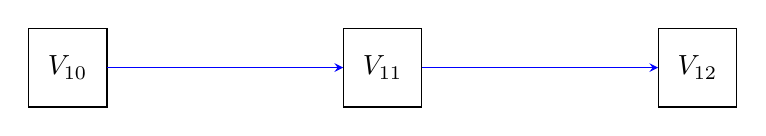
\begin{tikzpicture}[scale=1]
            \draw (0,0) rectangle (1,1);
            \node at (0.5,0.5) {$V_{10}$};
            \draw (4,0) rectangle (5,1);
            \node at (4.5,0.5) {$V_{11}$};
            \draw (8,0) rectangle (9,1);
            \node at (8.5,0.5) {$V_{12}$};
            \draw[blue,-stealth] (1,0.5) -- (4,0.5);
            \draw[blue,-stealth] (5,0.5) -- (8,0.5);
          \end{tikzpicture}
        \end{center}
        \begin{enumerate}
          \item Version 10 is finished and version 11 is in
            progress, but defects in version 10 must be fixed and
            released (as version $10.A$) before version 11 is
            ready. 
            \begin{solution}[1.45in]
            \end{solution}
          \item Version $10.A$ is merged into the main branch before
            version 11 is released.
            \begin{solution}[1.45in]
            \end{solution}
          \item Version 11 is completed and version 12 is in progress,
            but some developers are exploring a different approach to
            error handling (version $11.A$), which might be included in
            version 12, but might also be delayed until version 13.
            \begin{solution}[1.45in]
            \end{solution}
          \item The two developers working on version $11.A$ disagree
            on how best to proceed.  One finishes a smaller set of 
            changes (as version $11.B$) that are added before version
            12 is finished.  The other continues with a larger set of
            changes, now called version $11.C$, that will be added to
            version 13.
            \begin{solution}[1.45in]
            \end{solution}
        \end{enumerate}
        
      \item What seems harder, technically -- branching or merging?
        Explain why.
        \begin{solution}[1in]
          Branching is simply making a copy; easy! 
          Merging requires comparison of changes made to two sources; hard!
        \end{solution}

      \item One popular modern version control system is called 
        {\tt Git}. Because {\tt Git} is a {\it distributed} VCS, it
        it uses slightly different terminology from that developed above.
        Conduct some internet searches to determine the {\tt git} commands
        that would accomplish each of the following.
        \par\vskip 15pt
        \begin{enumerate}
          \itemsep 15pt
          \item Initialize a new repository
            \hfill\fillin[git init {\it project-name } ][2.25in]
          \item Create a local copy of a remote repository
            \hfill\fillin[git init {\it project-url } ][2.25in]
          \item Check the status of the files in your local repository
            \hfill\fillin[git status][2.25in]
          \item Add files to your local repository
            \hfill\fillin[git add {\it files} ][2.25in]
          \item Commit changes to your local repository
            \hfill\fillin[git commit -m {\it message} ][2.25in]
          \item Update your local repository from a remote repository
            \hfill\fillin[git pull ][2.25in]
          \item Send your local changes to the remote repository
            \hfill\fillin[git push][2.25in]
          \item Create a new branch in your local repository  
            \hfill\fillin[git branch {\it branch-name} ][2.25in]
        \end{enumerate}

  \end{enumerate}
       
\end{document}
